\documentclass[a4paper,11pt]{article}
\usepackage[czech]{babel}
\usepackage[utf8]{inputenc}
\usepackage[left=2cm, top=3cm, text={17cm, 24cm}]{geometry}
\usepackage{times}
\usepackage{multirow}
\usepackage[ruled, linesnumbered, noline, longend, czech]{algorithm2e}
\usepackage{graphics}
\usepackage[unicode]{hyperref}
\usepackage{pdflscape}
\usepackage{ctable}
\usepackage{csquotes}
    \MakeOuterQuote{"}
    \DeclareQuoteStyle{czech}
    {\quotedblbase}		
    {\textquotedblleft}	
    {\textquoteleft}	
    {\textquoteright}
    \setquotestyle{czech}

\setlength{\unitlength}{1mm}


\title{ITY_2}
\author{Václav Doleček}
\date{March 2019}

\begin{document}
\begin{titlepage}
\begin{center}
    \Huge
    \textsc{Vysoké učení technické v~Brně}\\
    \huge
    \textsc{Fakulta informačních technologií}\\
    \vspace{\stretch{0.382}}
    \Large
    Typografie a publikování-3.projekt\\
    \huge
    Tabulky a obrázky
    \vspace{\stretch{0.618}}
\end{center}
{\large 20.března.2019 \hfill Václav Doleček(xdolec03)}

\end{titlepage}

\newpage

\section{Úvodní strana}
Název práce umístěte do zlatého řezu a nezapomeňte uvést dnešní datum a vaše jmeno a příjmení.

\section{Tabulky}
Pro sázení tabulek můžeme použít buď prostředí \verb|tabbing| nebo prostředí \verb|tabular|.

\subsection{Prosředí \texttt{tabbing}}
Při použití \verb|tabbing| vypadá tabulka následovně:
\begin{tabbing}%
Vodní meloun \quad \= \textbf{cena}\quad \= \textbf{množství} \kill \\
\textbf{Ovoce}\quad \> \textbf{cena}\quad \> \textbf{množství} \\
jablka \> 25,00 \> 3kg
\\
Hrušky \> 27,40 \> 2,5kg
\\
Vodni meloun \> 35,-- \> 1kus
\\
\end{tabbing}

Toto prostředí se dá také použít pro sázení algoritmů, ovšem vhodnějsí je použít prostředí \verb|algorithm| nebo \verb|altorithm2e| (viz sekce3).

\subsection{Prostředí \texttt{tabular}}
Další možností, jak vytvořit tabulku, je použít prostředí \verb|tabular|. Tabulky pak budou vypadat takto\footnote{Kdyby byl problsem s~\texttt{cline}, zkuste se podívat třeba sem: http://www.abclinuxu.cz/tes/poradna/show/325037}:
\\
\begin{table}[h]
\begin{center}
\catcode`\-=12
\begin{tabular}{| l | c | r |}
      \hline  & \multicolumn{2}{c |} {\textbf{Cena}} \\
    \cline{2-3} \textbf{Měna} & \textbf{nakup} & \textbf{prodej} \\
    \cline{1-3}
    EUR & 25,615 & 27,20    \\
    GBP & 29,899 & 31,80 \\
    USD & 22,571 & 25,51 \\
     \hline
\end{tabular}
\\
\

Tabulka 1: Tabulka kurzů k~dnešnímu dni
\end{center}
\end{table}

\begin{table}[h]
    \begin{center}
    \catcode`\-=12
        \begin{tabular}{| c | c |}\hline
            $A$ & $\neg A$ \\ \hline
            \textbf{P} & N \\ \hline
            \textbf{O} & O~\\ \hline
            \textbf{X} & X \\ \hline
            \textbf{N} & P \\ \hline      
        \end{tabular}
        \begin{tabular}[p]{| c | c | c | c | c | c |}\hline
            \multicolumn{2}{| c |}{\multirow{2}{*}{$ A \wedge B$}} & \multicolumn{4}{c |}{$B$} \\ \cline{3-6}
            \multicolumn{2}{| c |}{} &  \textbf{P} & \textbf{O} & \textbf{X} & \textbf{N} \\ \hline
             \multirow{4}{*}{$A$} & \textbf{P} & P & O~& N & N \\ \cline{2-6}
             & \textbf{O} & O~& O~& N & N \\ \cline{2-6}
             & \textbf{X} & X & N & X & N \\ \cline{2-6}
             & \textbf{N} & N & N & N & N \\ \hline
        \end{tabular}
        \begin{tabular}[p]{| c | c | c | c | c | c |}\hline
            \multicolumn{2}{| c |}{\multirow{2}{*}{$ A \vee B$}} & \multicolumn{4}{c |}{$B$} \\ \cline{3-6}
            \multicolumn{2}{| c |}{} &  \textbf{P} & \textbf{O} & \textbf{X} & \textbf{N} \\ \hline
            \multirow{4}{*}{$A$} & \textbf{P} & P & P & P & P \\ \cline{2-6}
            & \textbf{O} & P & O~& P & O~\\ \cline{2-6}
            & \textbf{X} & P & P & X & X \\ \cline{2-6}
            & \textbf{N} & P & O~& X & N \\ \hline
        \end{tabular}
        \begin{tabular}[p]{| c | c | c | c | c | c |}\hline
            \multicolumn{2}{| c |}{\multirow{2}{*}{$ A \to B$}} & \multicolumn{4}{c |}{$B$} \\ \cline{3-6}
            \multicolumn{2}{| c |}{} &  \textbf{P} & \textbf{O} & \textbf{X} & \textbf{N} \\ \hline
            \multirow{4}{*}{$A$} & \textbf{P} & P & O~& X & N \\ \cline{2-6}
            & \textbf{O} & P & O~& P & O~\\ \cline{2-6}
            & \textbf{X} & P & P & X & X \\ \cline{2-6}
            & \textbf{N} & P & P & P & P \\ \hline
        \end{tabular}
    \end{center}
    Tabulka 2: Protože Kleeneho trojhodnotová logika už je "Zastaralá", uvádíme si zde příklad čtyřhodnotové \linebreak logiky
    
\end{table}
\pagebreak
\newpage

\section{Algoritmy}
Pokud budeme chtít vysázet algoritmus, můžeme použít prostředí \texttt{algorithm} \footnote{Pro nápovědu, jak zacházet s~prostředím\texttt{ algorithm, } můžeme zkusit tuhle stránku:\\\href{http://ftp.cstug.cz/pub/tex/CTAN/macros/latex/contrib/algorithms/algorithms.pdf}{http://ftp.cstug.cz/pub/tex/CTAN/macros/latex/contrib/algorithms/algorithms.pdf}} nebo \texttt{algorithm2e} \footnote{Pro \texttt{ algorithm2e }zase tuhle: \href{http://fip.cstug.cz/pub/tex/CTA/macros/latex/contrib/algorithm2e/algorithm2e.pdf}{http://fip.cstug.cz/pub/tex/CTA/macros/latex/contrib/algorithm2e/algorithm2e.pdf}}.\\
Příklad použití prostředí \verb|algorithm2e| viz Algoritmus \ref{alg:one}\\


\begin{algorithm}[H]
\caption{\textsc{FanstSLAM}}
\label{alg:one}

\SetNlSty{}{}{:}
\SetInd{1em}{1em}
\KwIn{$ (X_{t-1}, u_t, z_t) $}
\KwOut{ $X_t$ }
\Indp
\BlankLine
    $ \overline{X_t} = X_t = 0 $ \\
    \For{$ k = 1 \textrm{\emph{ to }} M $}{
    $ x_t^{[k]} = \emph{sample\_motion\_model}(u_t, x_{t - 1}^{[k]}) $ \\
    $ \omega_t^{[k]} = \emph{measurement\_model}(z_t, x_t^{[k]}, m_{t - 1}) $ \\
    $ m_t^{[k]} = updated\_occupancy\_grid(z_t, x_t^{[k]}, m_{t - 1}^{[k]}) $ \\
    $ \overline{X_t} = \overline{X_t} + \langle x_x^{[m]}, \omega_t^{[m]}  \rangle $ \\
    }
    \For{$ k = 1 \textrm{\emph{ to }} M $}{
    draw $ i $ with probability $ \approx \omega_t^{[i]} $ \\
    add $ \langle x_x^{[k]}, m_t^{[k]} \rangle \textrm{ to } X_t $ \\
    }    
    \Return{$ X_t $}
\end{algorithm}


\section{Obrázky}
Do našich článků můžeme samozřejmě vkládat obrázky. Pokud je obrázek fotografie, můžeme klidně použít bitmapový
soubor. Pokud by to ale mělo být nějaké schéma nebo néco podobného, je dobrým zvykem takovéto
obrázek vytvořit vektorově.

\begin{figure}[h]
\centering
    \scalebox{0.4}{
    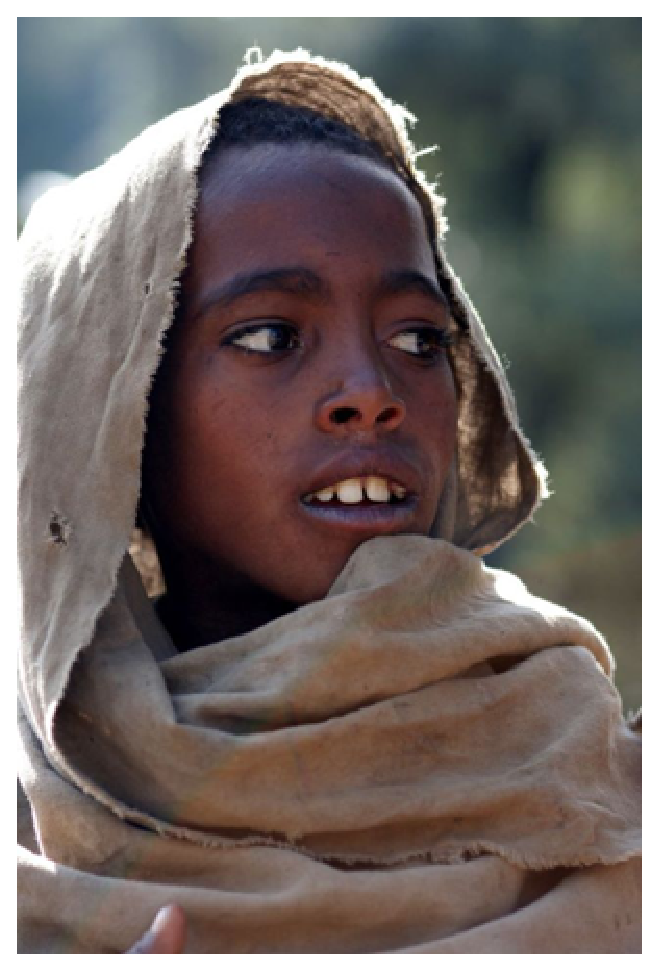
\includegraphics{etiopan.eps}
    \reflectbox{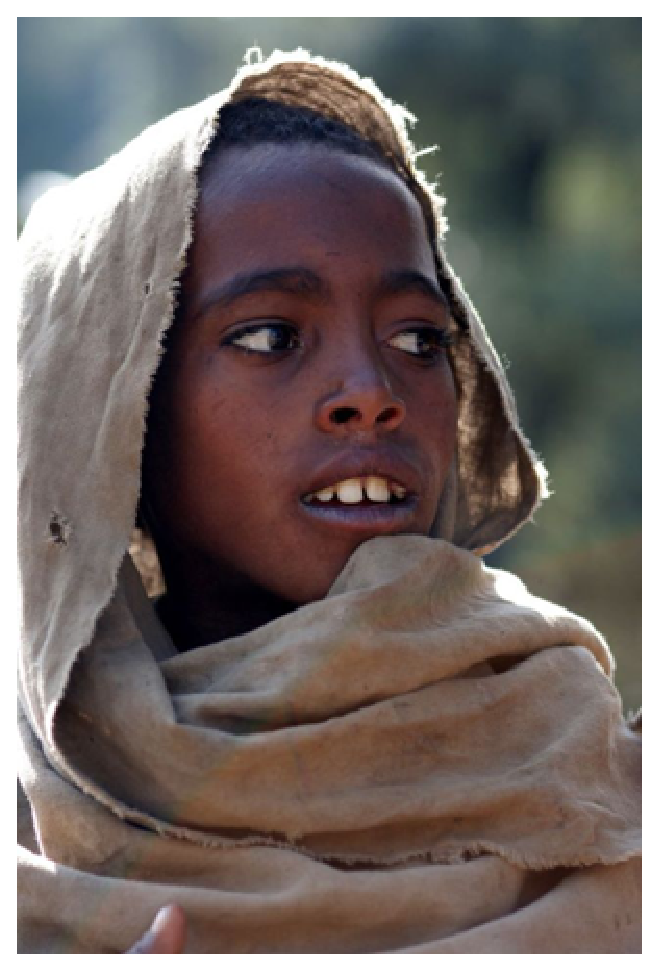
\includegraphics{etiopan.eps}}
    }
    \caption{Maly Etiopánek a jeho bratříček}
    \label{figure:etiopan}
\end{figure}
\newpage
Rozdíl mezi vektorový\dots
\begin{figure}[h]
    \scalebox{0.4}{
    
\includegraphics{oniisan.eps}
    }
    \centering
    \caption{Vektorý obrázek}
    \label{figure:oniisan.ep}
\end{figure}

\noindent\dots a birmapovým obrázkem

\begin{figure}[ht]
    \scalebox{0.6}{
    
\includegraphics{oniisan2.eps}
    }
    \centering
    \caption{Bitmapový obrázek}
    \label{figure:oniisan2.eps}
\end{figure}
\noindent se projeví například při zvětšení.

Odkazy (nejen ty) na obrázky 1, 2 a 3 a také na algoritmus 1 josu udělány pomocí křížových odkazů. Pak je ovšem potřeba zdrojový soubor přeložit dvakrát.

Vektorové obrázky lze vytvořit i přímo v~\LaTeX u, například pomocí prostředí \verb|picture.|

\newpage

\begin{landscape}
\begin{figure}[ht]
\begin{center}
    \begin{picture}(250, 150)
    \linethickness{1mm}
        \put(0,0){\framebox(250, 150){}}
        %souradnice utesu pod hradem
        \linethickness{0.1mm}
        \put(10,0){\line(1,5){5}}
        \put(15,25){\line(2,3){10}}
        \put(25,40){\line(4,-1){20}}
        \put(45,35){\line(6,1){30}}
        \put(75,40){\line(1,0){30}}
        \put(105,40){\line(1,2){5}}
        \put(110,50){\line(2,1){10}}
        \put(120,55){\line(1,-1){5}}
        \put(125,50){\line(2,-1){10}}
        \put(135,45){\line(1,-1){10}}
        \put(145,35){\line(1,-2){5}}
        \put(150,25){\line(0,-1){25}}
        %hrad
        \put(25,40){\line(0,1){25}}
        \put(25,65){\line(1,0){5}}
        \put(30,65){\line(0,-1){5}}
        \put(30,60){\line(1,0){5}}
        \put(35,60){\line(0,1){5}}
        \put(35,65){\line(1,0){5}}
        \put(40,65){\line(0,-1){5}}
        \put(40,60){\line(1,0){5}}
        \put(45,60){\line(0,1){5}}
        \put(45,65){\line(1,0){5}}
        \put(50,65){\line(0,-1){5}}
        \put(50,60){\line(1,0){5}}
        \put(55,60){\line(0,1){5}}
        \put(55,65){\line(1,0){5}}
        \put(60,65){\line(0,-1){5}}
        \put(60,60){\line(1,0){5}}
        \put(65,60){\line(0,1){5}}
        \put(65,65){\line(1,0){5}}
        \put(70,65){\line(0,-1){5}}
        \put(70,60){\line(1,0){5}}
        \put(75,60){\line(0,1){5}}
        \put(75,65){\line(1,0){5}}
        \put(80,65){\line(0,-1){5}}
        \put(80,60){\line(1,0){5}}
        \put(85,60){\line(0,1){5}}
        \put(85,65){\line(1,0){5}}
        \put(90,40){\line(0,1){35}}
        \put(85,75){\line(1,0){60}}
        \put(140,75){\line(0,-1){35}}
        \put(85,75){\line(2,1){10}}
        \put(95,80){\line(1,2){5}}
        \put(100,90){\line(1,0){30}}
        \put(130,90){\line(1,-2){5}}
        \put(135,80){\line(2,-1){10}}
        \put(100,65){\line(1,0){5}}
        \put(105,65){\line(0,1){5}}
        \put(105,70){\line(-1,0){5}}
        \put(100,70){\line(0,-1){5}}
        \put(125,65){\line(1,0){5}}
        \put(130,65){\line(0,1){5}}
        \put(130,70){\line(-1,0){5}}
        \put(125,70){\line(0,-1){5}}
        \put(45,65){\line(0,1){35}}
        \put(65,65){\line(0,1){35}}
        \put(40,100){\line(1,0){30}}
        \put(40,100){\line(0,1){30}}
        \put(70,100){\line(0,1){30}}
        \put(30,130){\line(1,0){50}}
        \put(30,130){\line(2,1){10}}
        \put(40,135){\line(1,2){5}}
        \put(45,145){\line(1,0){20}}
        \put(65,145){\line(1,-2){5}}
        \put(70,135){\line(2,-1){10}}
        %breh
        \put(180,0){\line(0,1){25}}
        \put(180,25){\line(1,2){5}}
        \put(185,35){\line(1,1){5}}
        \put(190,40){\line(1,0){60}}
        %most
        \put(150,25){\line(1,1){5}}
        \put(155,30){\line(2,1){10}}
        \put(165,35){\line(2,-1){10}}
        \put(175,30){\line(1,-1){5}}
        \put(140,40){\line(1,0){50}}
        \put(140,45){\line(1,0){50}}
        \put(150,45){\line(0,-1){5}}
        \put(160,45){\line(0,-1){5}}
        \put(170,45){\line(0,-1){5}}
        \put(180,45){\line(0,-1){5}}
        \put(190,40){\line(0,1){20}}
        \put(205,40){\line(0,1){20}}
        \put(185,60){\line(1,0){25}}
        \put(185,60){\line(0,1){10}}
        \put(185,70){\line(1,0){5}}
        \put(190,70){\line(0,-1){5}}
        \put(190,65){\line(1,0){5}}
        \put(195,65){\line(0,1){5}}
        \put(195,70){\line(0,-1){5}}
        \put(195,70){\line(1,0){5}}
        \put(200,70){\line(0,-1){5}}
        \put(200,65){\line(1,0){5}}
        \put(205,65){\line(0,1){5}}
        \put(205,70){\line(1,0){5}}
        \put(210,70){\line(0,-1){10}}
        \put(55, 115){\circle{10}}
    \end{picture}
    \caption{Vektorový obrázek pevnosti "Krkavčí Hnízdo" dle mého vlastního návrhu}
\end{center}
\end{figure}
\end{landscape}

\end{document}

